\subsection{\textit{Set}: Grouping and Compositionality in Relational Reasoning}\label{ssec:experiments_set}

\textit{Set} is a card game that forms a simple-to-describe but challenging relational task. The `objects' are a set of cards with four attributes, each of which can take one of three possible values. `Color' can be red, green, or purple; `number' can be one, two, or three; `shape' can be diamond, squiggle, or oval; and `fill' can be solid, striped, or empty. A `set' is a triplet of cards such that each attribute is either a) the same on all three cards, or b) different on all three cards.

\begin{figure}[ht]
    \vskip-10pt
    \centering
    \begin{subfigure}[b]{0.49\textwidth}
        \centering
        \raisebox{20pt}{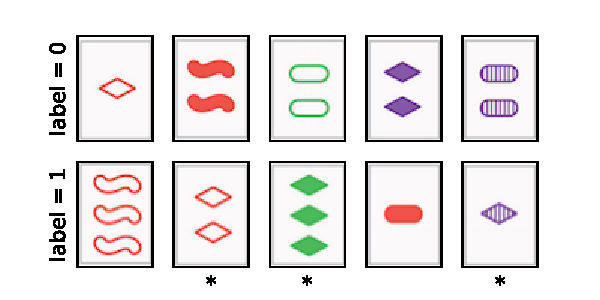
\includegraphics[width=\textwidth]{figs/contains_set_example.pdf}}
        \caption{Example of ``contains set'' task.}\label{fig:contains_set_example}
    \end{subfigure}
    \begin{subfigure}[b]{0.5\textwidth}
        \centering
        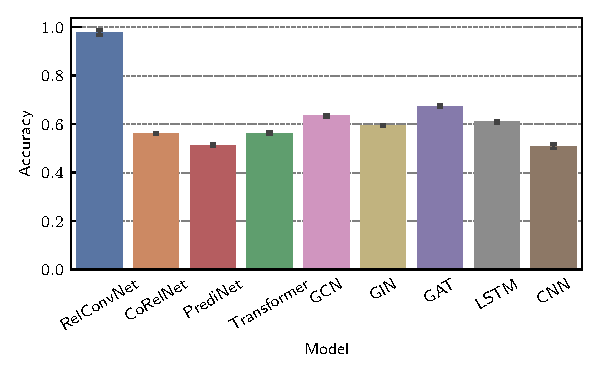
\includegraphics[width=\textwidth]{figs/experiments/contains_set_acc_tunedbaselines.pdf}
        \vskip-5pt
        \caption{\footnotesize{Hold-out test accuracy.}}\label{fig:contains_set_acc}
    \end{subfigure}

    \begin{subfigure}[t]{0.97\textwidth}
        \centering
        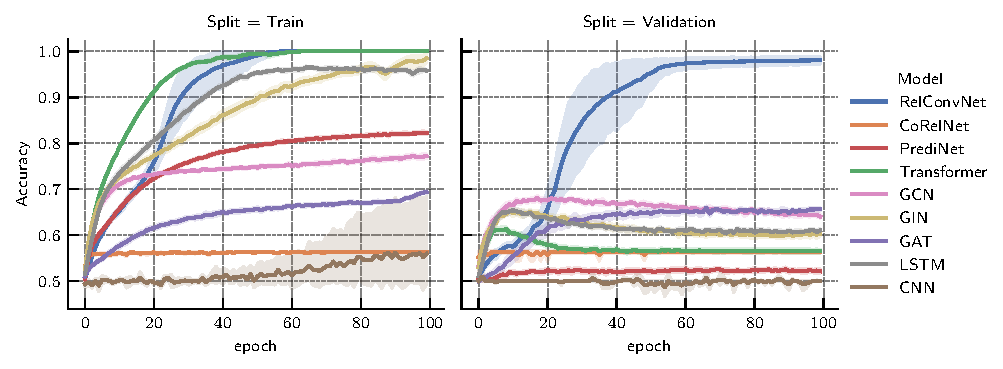
\includegraphics[width=0.975\textwidth]{figs/experiments/contains_set_training_curves_tunedbaselines.pdf}
        \caption{Training accuracy and validation accuracy over the course of training.}\label{fig:contains_set_training_curves}
    \end{subfigure}
    % \begin{subfigure}[t]{0.45\textwidth}
    %     \centering
    %     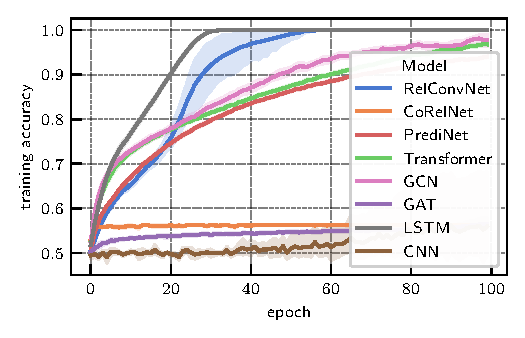
\includegraphics[width=0.9\textwidth]{figs/experiments/contains_set_training_curves_trainacc.pdf}
    %     \vskip-5pt
    %     \caption{Training accuracy over the course of training.}\label{fig:contains_set_training_curves_trainacc}
    % \end{subfigure}
    % \begin{subfigure}[t]{0.45\textwidth}
    %     \centering
    %     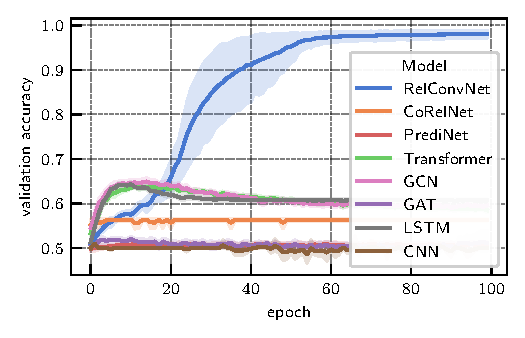
\includegraphics[width=0.9\textwidth]{figs/experiments/contains_set_training_curves_valacc.pdf}
    %     \vskip-5pt
    %     \caption{Validation accuracy over the course of training.}\label{fig:contains_set_training_curves_valacc}
    % \end{subfigure}
    \caption{Results of ``contains set'' experiments. Bar height/solid lines indicate the mean over 10 trials and error bars/shaded regions indicate 95\% bootstrap confidence intervals.}\label{fig:contains_set_experiment}
    \vskip-5pt
\end{figure}

% \begin{figure}[ht]
%     \centering
%     \begin{minipage}{0.49\textwidth}
%         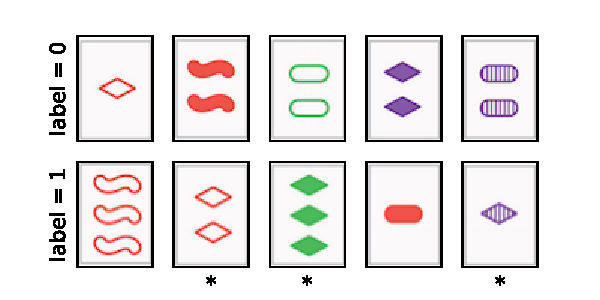
\includegraphics[width=0.9\textwidth]{figs/contains_set_example.pdf}
%         \caption{Example of the ``contains set'' task.}\label{fig:contains_set_example}
%     \end{minipage}
%     \begin{minipage}{0.49\textwidth}
%         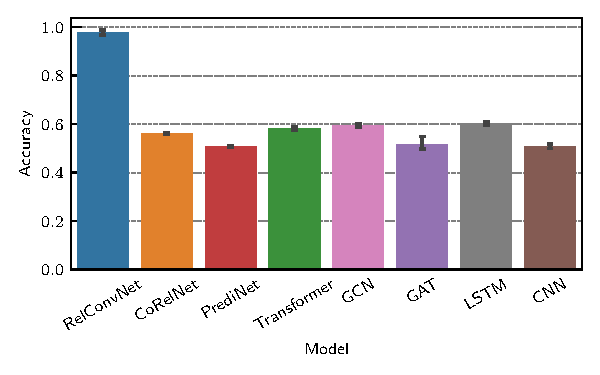
\includegraphics[width=0.9\textwidth]{figs/experiments/contains_set_acc.pdf}
%         \caption{Hold-out test accuracy. Bar height indicates mean over 10 trials and error bars indicate 95\% confidence intervals.}\label{fig:contains_set_acc}    
%     \end{minipage}
% \end{figure}

% \begin{figure}[ht]
%     \centering
%     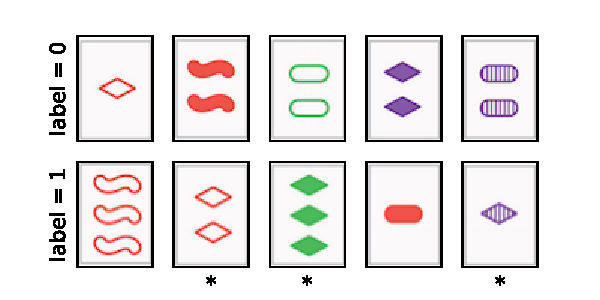
\includegraphics[width=0.4\textwidth]{figs/contains_set_example.pdf}
%     \vskip-12pt
%     \caption{Example of the ``contains set'' task.}\label{fig:contains_set_example}
%     \vskip-7pt
% \end{figure}

In \textit{Set}, the task is: given a hand of $n > 3$ cards, find a `set' among them.~\Cref{fig:contains_set_example} depicts a positive and negative example for $n=5$, with $*$ indicating the `set' in the positive example.
% (typically, \textit{Set} is played with $k=12$, with two players competing to find a `set' first). 
This task is deceptively challenging, and is representative of the type of relational reasoning that humans excel at but machine learning systems still struggle with. To solve the task, one must process the sensory information of individual cards to identify the values of each attribute, and then reason about the relational pattern in each triplet of cards.
% Importantly, this type of relational reasoning requires attending over several attributes and relations simultaneously while representing some notion of `groups'.  
The construct of relational convolutions proposed in this paper is a step towards developing machine learning systems that can perform this kind of relational reasoning.

% \begin{figure}[ht]
%     \centering
%     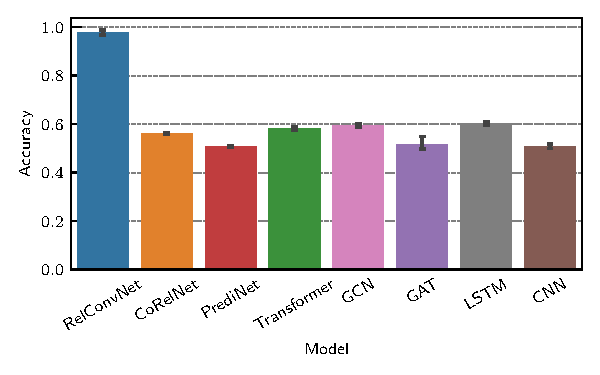
\includegraphics[width=0.4\textwidth]{figs/experiments/contains_set_acc.pdf}
%     % \vskip-12pt
%     \caption{Hold-out test accuracy. Bar height indicates mean over 10 trials and error bars indicate 95\% confidence intervals.}\label{fig:contains_set_acc}
%     % \vskip-10pt
% \end{figure}

In this section, we evaluate RelConvNet on a task based on \textit{Set} and compare it to several baselines. The task is: given a collection of $n=5$ images of \textit{Set} cards, determine whether or not they contain a `set'. All models share the common architecture $(x_1, \ldots, x_n) \to \texttt{CNN} \to \{ \cdot \} \to \texttt{MLP} \to \hat{y}$, where $\{\cdot\}$ indicates the central module being tested.
% In addition to CoRelNet, PrediNet, and Transformers, we also compare RelConvNet to several GNN baselines. 
The CNN embedder is pre-trained on the task of classifying the four attributes of the cards and an intermediate layer is used to generate embeddings. The output MLP architecture is shared across all models.
%  of dimension $64$ for each card. The output MLP architecture is shared across all models, and consists of two hidden layers with $64$ and $32$ neurons, respectively, and ReLU activations. 
Further architectural details can be found in~\Cref{sec:experiments_supplement}. 

% \begin{figure}[t]
%     \centering
%     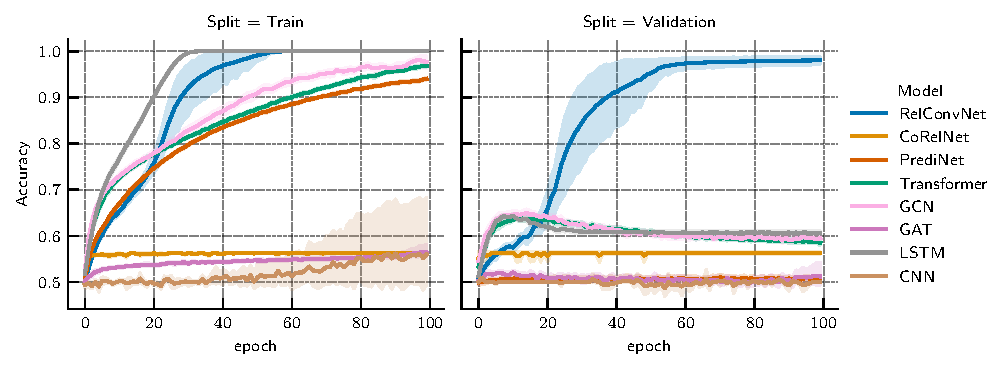
\includegraphics[width=0.8\textwidth]{figs/experiments/contains_set_training_curves.pdf}
%     % \vskip-10pt
%     \caption{Training accuracy and validation accuracy over the course of training. Solid lines indicate mean over 10 trials and shaded regions indicates 95\% bootstrap confidence intervals.}\label{fig:contains_set_training_curves}
%     % \vskip-12pt
% \end{figure}

In \textit{Set}, there exists $\binom{81}{3} = 85\,320$ triplets of cards, of which $1\,080$ are a `set'. We partition the `sets' into training (70\%), validation (15\%), and test (15\%) sets. The training, validation, and test datasets are generated by sampling $n$-tuples of cards such that with probability $1/2$ the $n$-tuple does not contain a set, and with probability $1/2$ it contains a set among the corresponding partition of sets. Partitioning the data in this way allows us to measure the models' ability to ``learn the rule'' and identify new unseen `sets'.
We train for 100 epochs with the same loss, optimizer, and batch size as the experiments in the previous section. For each model, we run 10 trials with different random seeds.

When using the default optimizer hyperparameters as in the previous experiment without hyperparameter tuning, we find that RelConvNet is the only model able to meaningfully learn the task in a manner that generalizes to unseen `sets'. In particular, we observe that many baselines severely overfit to the training data, failing to learn the rule and generalize (see~\Cref{ssec:set_no_hyperparameter_sweep}). Although RelConvNet did not require hyperparameter tuning, we carry out an extensive hyperparameter sweep for all other baselines individually in order to validate our conclusions against the best-achievable performance for each baseline. We ran a total of 1600 experimental runs searching over combinations of architectural hyperparameters (number of layers) and optimization hyperparameters (weight decay, learning rate schedule) individually for each baseline, with the goal of finding a hyperparameter configuration that is representative of the best achievable performance for each model class on this task. The results of the hyperparameter sweep are summarized in~\Cref{sec:baseline_hyperparameter_sweep}.

\Cref{fig:contains_set_acc} shows the hold-out test accuracy for each model.~\Cref{fig:contains_set_training_curves} shows the training and validation accuracy over the course of training. Here, RelConvNet uses the Adam optimizer with the default Tensorflow hyperparameters (constant learning rate of $0.001$, $\beta_1 = 0.9, \beta_2 = 0.999$) while each baseline has its own individually-optimized hyperparameters, described in~\Cref{sec:baseline_hyperparameter_sweep}.

We observe a sharp separation between RelConvNet and all other baselines. While RelConvNet is able to learn the task and generalize to new `sets' with near-perfect accuracy (avg: 97.9\%), no other model is able to reach a comparable generalization accuracy even after hyperparameter tuning. The next best is the GAT model (avg: 67.5\%). Several models are able to fit the training data, reaching near-perfect training accuracy, but they are unable to ``learn the rule'' in a way that generalizes to the validation or test sets. This suggests that while these models are powerful function approximators, they lack the \textit{inductive biases} to learn hierarchical relations.

\begin{wrapfigure}{r}{0.5\textwidth}
    \centering
    \vskip-10pt
    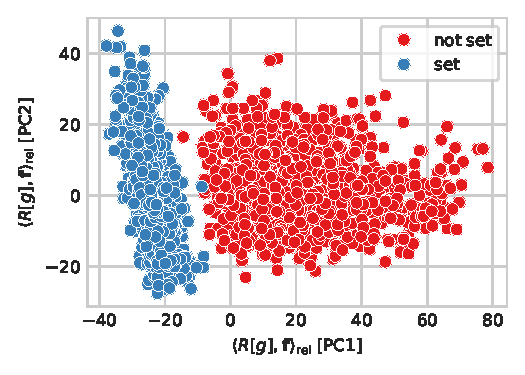
\includegraphics[width=0.5\textwidth]{figs/representation_analysis/conv_rep.pdf}
    \caption{The relational convolution layer produces representations that separates `sets' from `non-sets'.}\label{fig:conv_rep}
    \vskip-5pt
\end{wrapfigure}

In~\Cref{fig:conv_rep} we analyze the geometry of the representations learned by the relational convolution layer. We consider all triplets of cards, compute the relation subtensor using the learned MD-IPR layer, and plot the relational inner product with the learned graphlet filter $\bm{f} \in \reals^{s \times s \times d_r \times n_f}$. The result is a $n_f$-dimensional vector for each triplet of cards. We perform PCA to plot this in two dimensions, and color-code each triplet of cards according to whether or not it forms a `set'. We find that the relational convolution layer learns a representation of the relational pattern in groups of objects that separates `sets' and `non-sets'. In particular, the two classes form clusters that are linearly separable even when projected down to two dimensions by PCA. This explains why RelConvNet is able to learn the task in a way that generalizes while the other models are not. In~\Cref{sec:appendix_rep_analysis} we expand on this discussion, and further analyze the representations learned by the MD-IPR layer, showing that the learned relations map to the color, number, shape, and fill attributes.

It is perhaps surprising that models like GNNs and Transformers perform poorly on these relational tasks, given their apparent ability to process relations through neural message-passing and attention, respectively. We remark that GNNs operate in a different domain compared to relational models like RelConvNe, PrediNet, and CoRelNet. In GNNs, the relations are an input to the model, received in the form of a graph, and are used to dictate the flow of information in a neural message-passing operation. By contrast, in relational convolutional networks, the input is simply a set of objects without relations---the relations need to be \textit{inferred} as part of the feature representation process. 
Thus, GNNs operate in domains where relational information is already present (e.g., analysis of social networks, biological networks, etc.), whereas our framework aims to solve tasks that rely on relations but those relations need to be inferred end-to-end. 
This offers a partial explanation for the inability of GNNs to learn this task---GNNs are good at processing network-style relations when they are given as input, but may not be able to infer and hierarchically process relations when they are not given. In the case of Transformers, relations are modeled implicitly to direct information retrieval in attention, but are not encoded explicitly in the final representations. By contrast, RelConvNet operates on collections of objects and possesses inductive biases for learning iteratively more complex relational representations, guided only by the supervisory signal of the downstream task. 

Models like CoRelNet and PrediNet have relational inductive biases, but lack compositionality. On the other hand, deep models like Transformers and GNNs are compositional, but lack relational inductive biases. This experiment suggests that \textit{compositionality and relational inductive biases are both necessary ingredients to efficiently learn representations of higher-order relations}. RelConvNet is a compositional architecture imbued with relational inductive biases and a demonstrated ability to tackle hierarchical relational tasks.
